\section{系统案例与讨论}

\subsection{从采集链路到决策支持}

本文的案例不是对某个产品已经成功落地的证明，而是展示系统如何把公开文本转成可追溯的决策候选。决策者可以先查看来源规模和正文质量，再查看代理复核中的原模型、盲复核和裁定差异，最后查看主题成员、来源覆盖和价值维度。这样的顺序把“记录是否构成机会”和“机会是否值得优先研究”分开，减少单一热度指标对决策的支配。图~\ref{fig:proxyconfusion} 展示全批次 2,561 条混合代理结果相对原模型的四类标签变化，其中 2,052 条未抽样记录沿用原标签。

\begin{figure}[H]
  \centering
  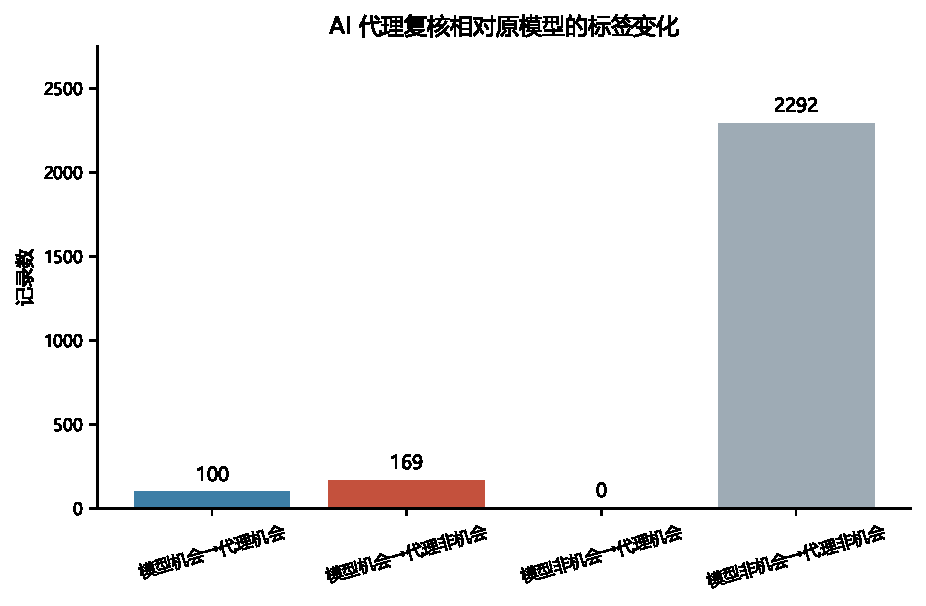
\includegraphics[width=0.82\textwidth]{../figures/fig06_proxy_confusion.pdf}
  \caption{混合代理结果相对原模型的标签交叉。四类共计 2,561 条；其中未抽样记录的标签沿用原模型，仅 509 条使用 AI 代理复核标签。}
  \label{fig:proxyconfusion}
\end{figure}

\subsection{数据与方法限制}

第一，来源之间的记录量和内容类型不均衡，Hacker News 占 B01 清洗记录的大部分，中文资讯和 RSS 历史覆盖有限。第二，部分记录只有标题、简介或短文本，907 条记录没有热度值，互动信号只能用于有数据的子集。第三，复核队列中的负例是面向难例的定向抽样，不能直接推断全量负例表现。第四，AI 代理裁定仍由同一模型完成，并且裁定输入包含此前模型输出，存在相关性与锚定风险。第五，主题轮廓系数较低、单记录主题较多，主题命名和功能行业众数不能替代人工主题边界判断。

因此，本文不报告经过人工真值验证的分类指标，也不把代理候选主题当成稳定市场热点。两轮复核与再次裁定均由同一 Codex 模型完成，结果只用于敏感性分析和系统链路验证，不能替代真人标注。正式比赛结果仍需要真人按统一标准确认至少全部预测机会记录，并对负例采用可解释的分层随机抽样，之后再生成正式 result2、result3 和 result4。系统已保留原始来源、处理配置、模型输出和代理裁定，能够在确认标签后重跑后续步骤。

\subsection{C2 候选方向的策划案框架}

C2 是当前代理评分最高的候选主题，包含 22 条记录，覆盖 GitHub、V2EX 和量子位三个来源，价值分为 85.76。成员标题涉及智能体架构、网络排障、医疗协同、代码模型和三维编辑等不同场景，因此 C2 的名称只能作为共同技术线索，不能直接等同于单一产品需求。

在证据边界内，C2 可形成待确认的策划案框架：目标是为需要多步骤知识检索、任务编排和结果回溯的团队提供可审计的智能体工作台；最小功能包括来源证据检索、任务分解与编排、过程日志、人工确认节点和结果引用；技术路线包括多语言向量检索、结构化模型调用、权限隔离与证据存储。上线前应以真人确认的需求记录为入口，比较引用正确率、任务完成时间和人工修改量，并对医疗等高风险场景单独设置人工审批。上述内容是由 C2 成员归纳出的实施假设，不是 B01 已观测到的用户承诺或产品效果。
